\subsubsection{Lunar Farside Location}
The lunar farside is a unique location in the inner solar system in that it is the only area that never faces the Earth due to tidal locking.  This means that it is only blocked from terrestial and near-terrestrial radio frequency transmissions.  This importance was recognized in the 1970's and the International Telecommunication Union (ITU\footnote{The ITU is the international organization that handles electromagnetic emission across national boundaries.} defined the Shielded Zone of the Moon (SZM) as “ compris[ing] the area of the Moon’s surface and an adjacent volume of space which are shielded from emissions originating within a distance of 100,000 km from the center of the Earth” \citep{ITU REGULATION}.

Near to the center Lunar Farside of -23.78930°N, 182.13737°E is essential to read signals of desired strength. Retaining a field of regard is less than 2 pi hemisherical for payload instruments. That near previously named and published LuSEE Night Landing site. Situated on a local elevated lunar feature, allowing maximum potential field of view. The Equatorial Fareside region will be home to Lunar day and Lunar night, both equating roughly equal to 14 days. Leading to ranges in survival temperture range of 213 to 348 K. With operational temperature ranges from 218 to 333 K.

    
\begin{figure}
	\centering
	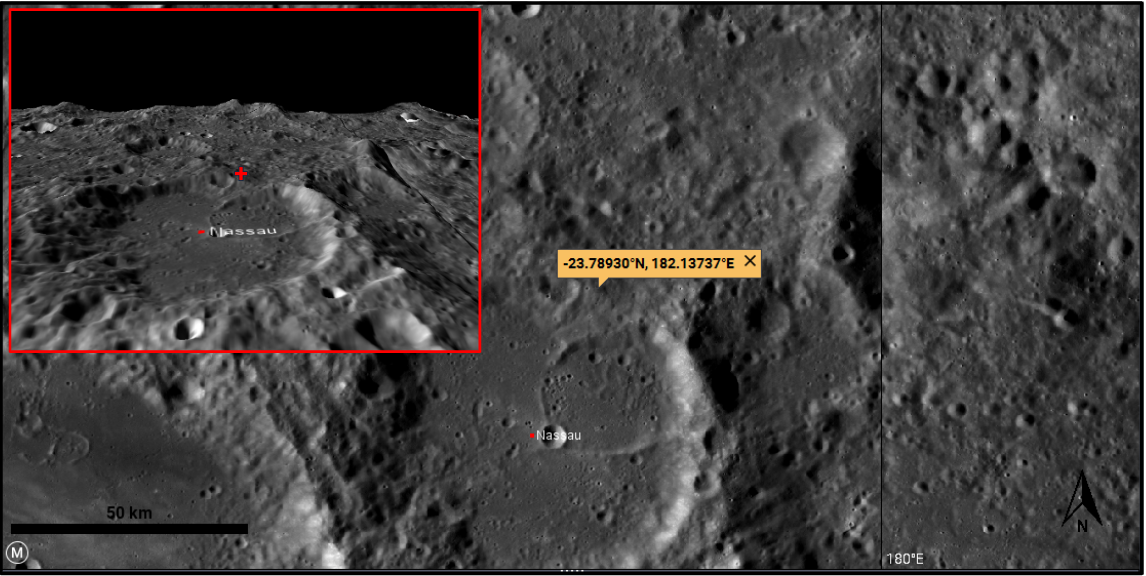
\includegraphics[width=\linewidth]{figures/Landing site overview.PNG}
	\caption{LFT3 Farside Landing Site - Micro View JMARS}
\end{figure}


\subsection{Site Regolith Conditions}
\textit{Study needed}
Regolith characteristics of the site are well known, to include regolith of no larger than X? size. Allowing proper landing conditions to exist for touchdown and operations. Not obstructing landing operations in depth, to include power down and gimbling. Upon initial touchdown the lander will experience expected position settling onto the regolith surface. Regolith characteristics will impact the final field of regard. Mission requirement of measuring the lander tilt will be taken once in position, on the lunar surface, for calibrated data.